\documentclass[11pt, a4paper]{article}
\usepackage[dutch]{babel}
\usepackage{graphicx}
\usepackage{subcaption}
\usepackage{wrapfig}
\usepackage{fullpage}
\usepackage{fancyhdr}
\usepackage{setspace}
\usepackage{color}
\usepackage{float}
\usepackage[parfill]{parskip}
\usepackage{listings}
\usepackage{color}
\usepackage{framed}
\definecolor{dkgreen}{rgb}{0,0.6,0}
\definecolor{gray}{rgb}{0.4,0.4,0.4}
\definecolor{mauve}{rgb}{0.58,0,0.82}

\lstset{
  language=R,                     % the language of the code
  basicstyle=\footnotesize,       % the size of the fonts that are used for the code
  numbers=left,                   % where to put the line-numbers
  numberstyle=\tiny\color{gray},  % the style that is used for the line-numbers
  stepnumber=1,                   % the step between two line-numbers. If it's 1, each line
                                  % will be numbered
  numbersep=12pt,                 % how far the line-numbers are from the code
  backgroundcolor=\color{white},  % choose the background color. You must add \usepackage{color}
  showspaces=false,               % show spaces adding particular underscores
  showstringspaces=false,         % underline spaces within strings
  showtabs=false,                 % show tabs within strings adding particular underscores
  rulecolor=\color{black},        % if not set, the frame-color may be changed on line-breaks within not-black text (e.g. comments (green here))
  tabsize=2,                      % sets default tabsize to 2 spaces
  captionpos=b,                   % sets the caption-position to bottom
  breaklines=false,               % sets automatic line breaking
  breakatwhitespace=false,        % sets if automatic breaks should only happen at whitespace
  title=\lstname,                 % show the filename of files included with \lstinputlisting;
                                  % also try caption instead of title
  keywordstyle=\color{blue},      % keyword style
  commentstyle=\color{dkgreen},   % comment style
  stringstyle=\color{mauve},      % string literal style
  linewidth=\textwidth            % if you want to add more keywords to the set
}

\pagestyle{fancyplain} {
	\fancyhead[L,R]{\thepage}
	\fancyhead[R,L]{Titouan Vervack}
}

\pagestyle{fancy}
\fancyhead{} % clear all header fields
\renewcommand{\headrulewidth}{0pt} % no line in header area
\fancyfoot{} % clear all footer fields
\fancyhead[LE,R]{\thepage}
\fancyhead[RE,L]{Titouan Vervack}
\setlength{\headsep}{15pt}

\begin{document}
\title{Statistische gegevensanalyse \\ Project}
\author{Titouan Vervack\\ Bachelor of Science in Informatics}
\date{31 mei 2014}
\maketitle
\newpage
\begin{wrapfigure}{r}{0.5\textwidth}
	\begin{center}
		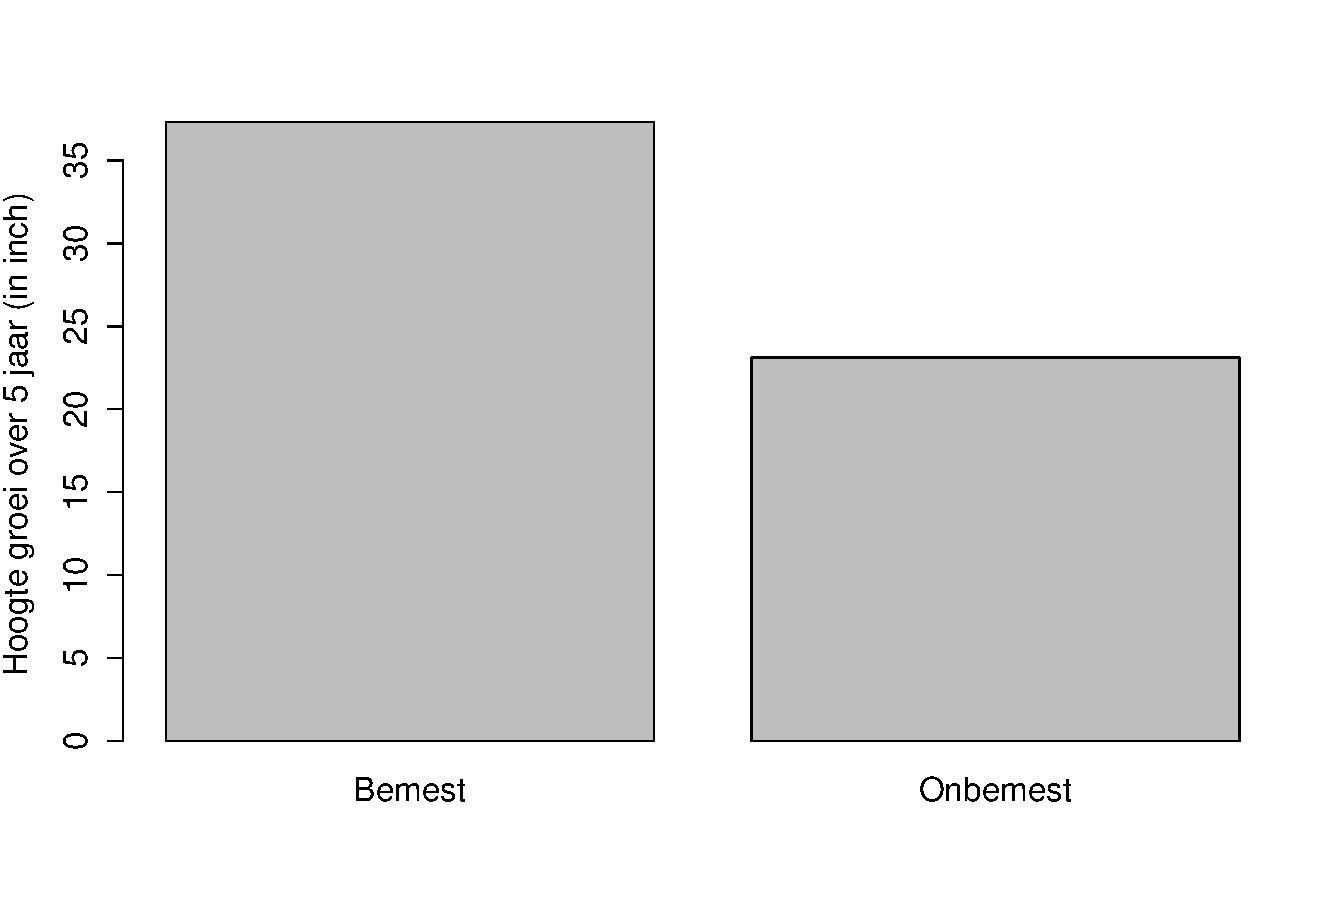
\includegraphics[scale=0.45]{barplot_a.pdf}
		\caption{Hoogte groei met bemesting of zonder bemesting}
		\label{bara}
		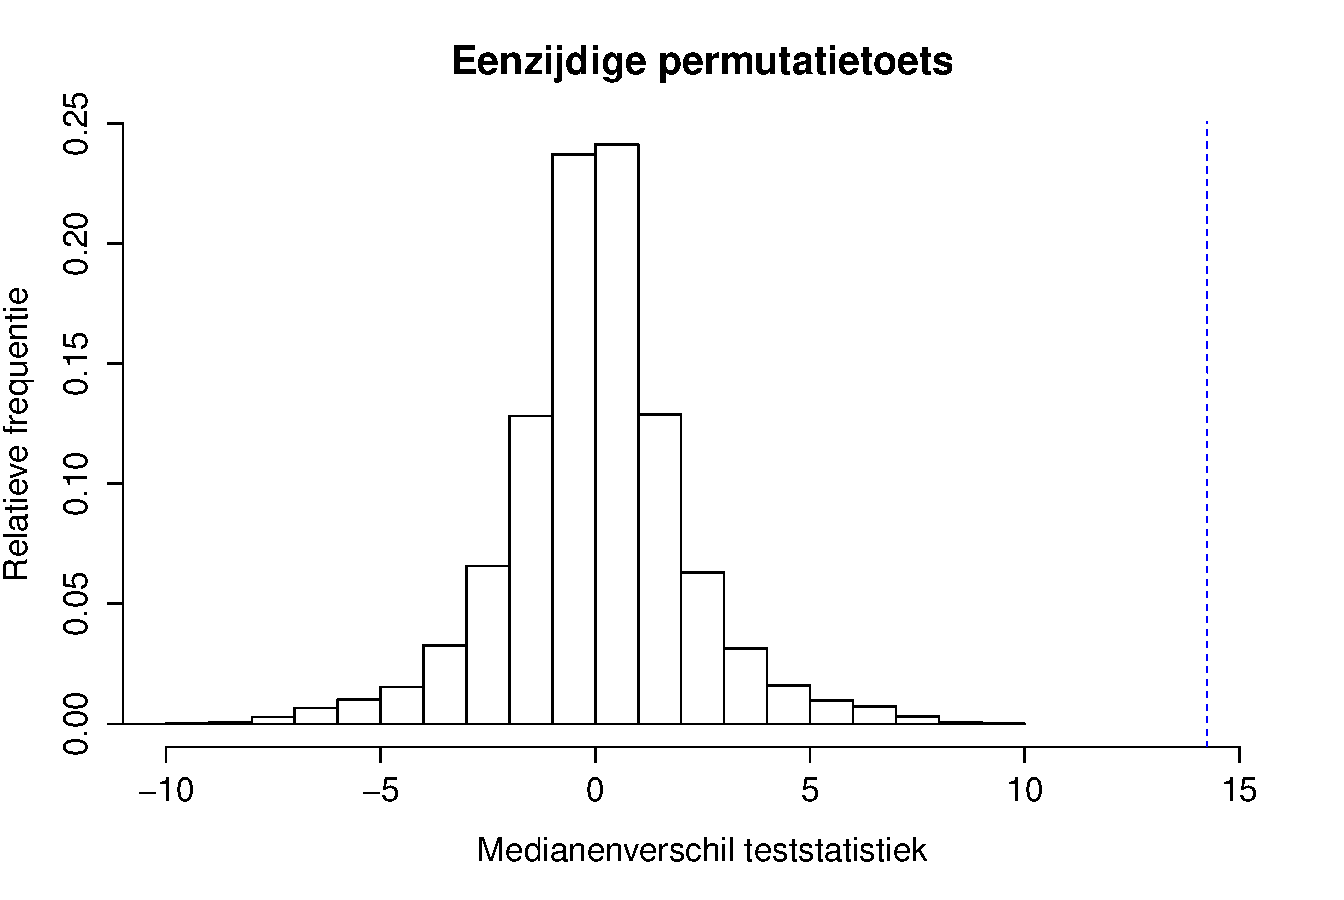
\includegraphics[scale=0.45]{perm_a.pdf}
		\caption{Permutatieverdeling voor de hoogte groei van (on)bemeste bomen}
		\label{perma}
		\vspace{0.5cm}
	\end{center}
\end{wrapfigure}
\section*{Opgave 1}
\subsection*{a}
Om de groei in hoogte van de bomen te bekijken trekken we \textbf{Height0} af van \textbf{Height5}. Aangezien gevraagd wordt wat de invloed is van bemesting op deze hoogte, gebruiken we dit in combinatie met \textbf{Fertilizer}. Om een beeld te krijgen van de data maken we er histogrammen van, we kiezen histogrammen omdat de hoogtes continue variabelen zijn. We kunnen zien dat de data niet symmetrisch is en pieken bevat. We kiezen daarom om de mediaan te gebruiken in plaats van het gemiddelde. In figuur \ref{bara} zien we de staafdiagram die deze medianen voorstelt, we zien dat bemesting een positief effect heeft op de hoogte groei van bomen. Om zeker te zijn dat dit effect wordt veroorzaakt door de bemesting voeren we een permutatietoets uit, dit is een eenzijdige toets aangezien gevraagd wordt of de bomen sneller groeien bij bemesting. $H_0$ stelt dat de groei bij geen of wel bemesting dezelfde is. $H_A$ stelt dat de groei bij bemesting positief is. De p-waarde, verkregen uit de permutatietoets, is $10^{-5}$. Dit is een overtuigend bewijs tegen de nulhypothese waardoor we deze mogen verwerpen ten voordele van de alternatieve hypothese. Bemesting heeft dus een positief effect op de hoogte groei van bomen. De permutatieverdeling op basis van $M = 99999$ is te zien in figuur \ref{perma}. % TODO: summary vergelijking 
\subsection*{b}
% Dirty hack to fix layout after using wrapfigures
\begin{wrapfigure}{R}{0pt}
\end{wrapfigure}
Bij deze opgave gebruiken we het verschil tussen \textbf{Diameter5} en \textbf{Diameter0}, we gebruiken ook \textbf{Competition}. 
We maken opnieuw histogrammen en beslissen om dezelfde reden terug de mediaan te gebruiken. De staafdiagram die de medianen vergelijkt is te zien in figuur \ref{barb}. Geen competitie blijkt een positief effect te hebben op de diameter van de bomen. We voeren ook hier een permutatietoets uit, dit is een tweezijdige aangezien het gevraagde effect niet gespecificeerd is. Om deze reden vermenigvuldigen we onze p-waarde met een factor $2$. $H_0$ stelt dat de groei bij geen of wel competitie gelijk is. $H_A$ stelt dat de groei bij geen of wel competitie niet gelijk is. De nulhypothese wordt verworpen door een terug lage p-waarde ten voordele van de alternatieve hypothese. Competitie verwijderen is dus positief voor de diameter van de bomen. De permutatieverdeling op basis van $M = 99999$ is te zien in figuur \ref{permb}. % TODO: summary vergelijking
\begin{figure}[H]
	\begin{center}
		\begin{subfigure}{0.49\textwidth}
			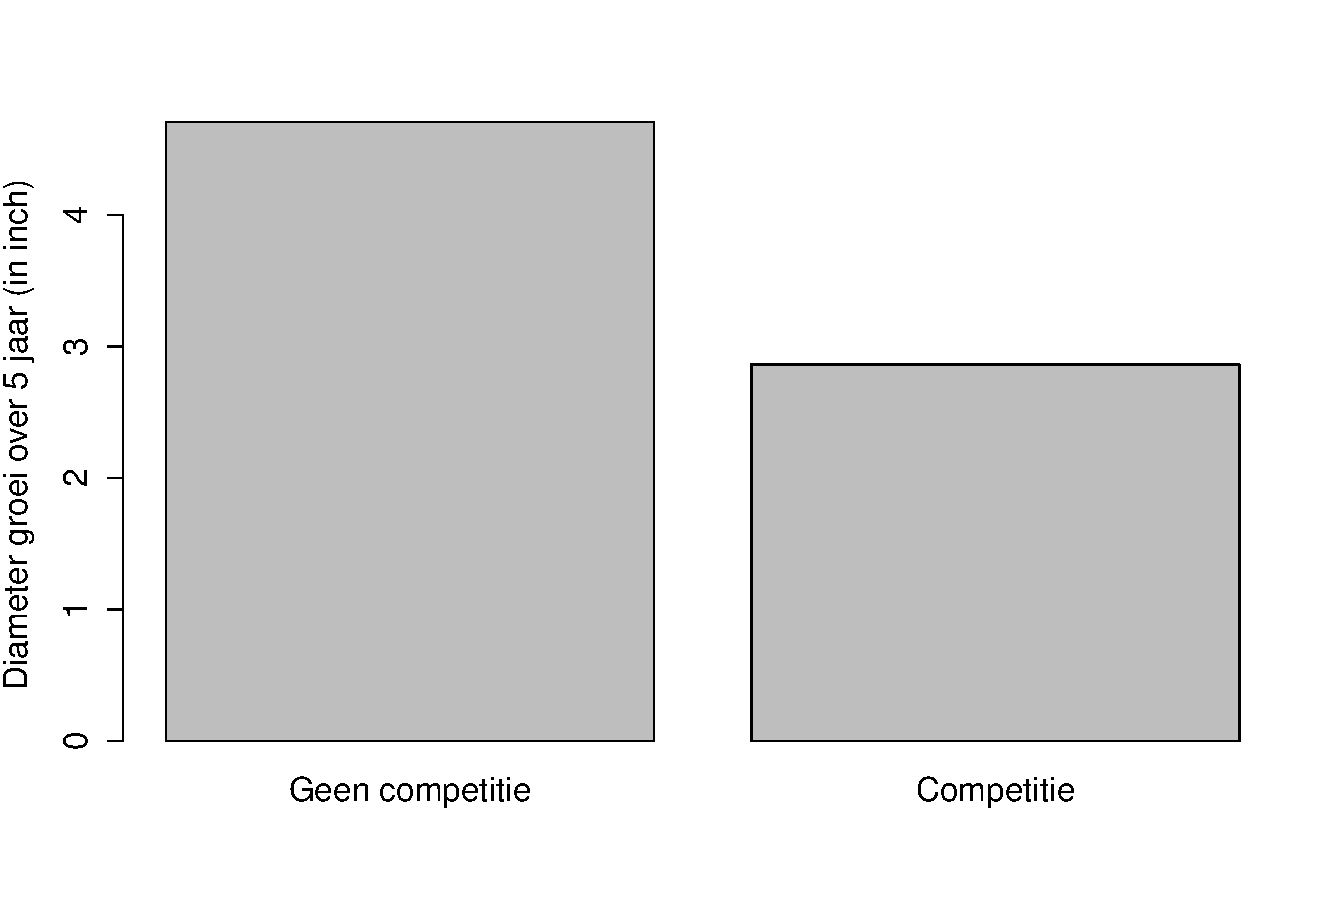
\includegraphics[scale=0.35]{barplot_b.pdf}
			\caption{Diameter groei met competitie of zonder competitie}
			\label{barb}
		\end{subfigure}
		\begin{subfigure}{0.49\textwidth}
			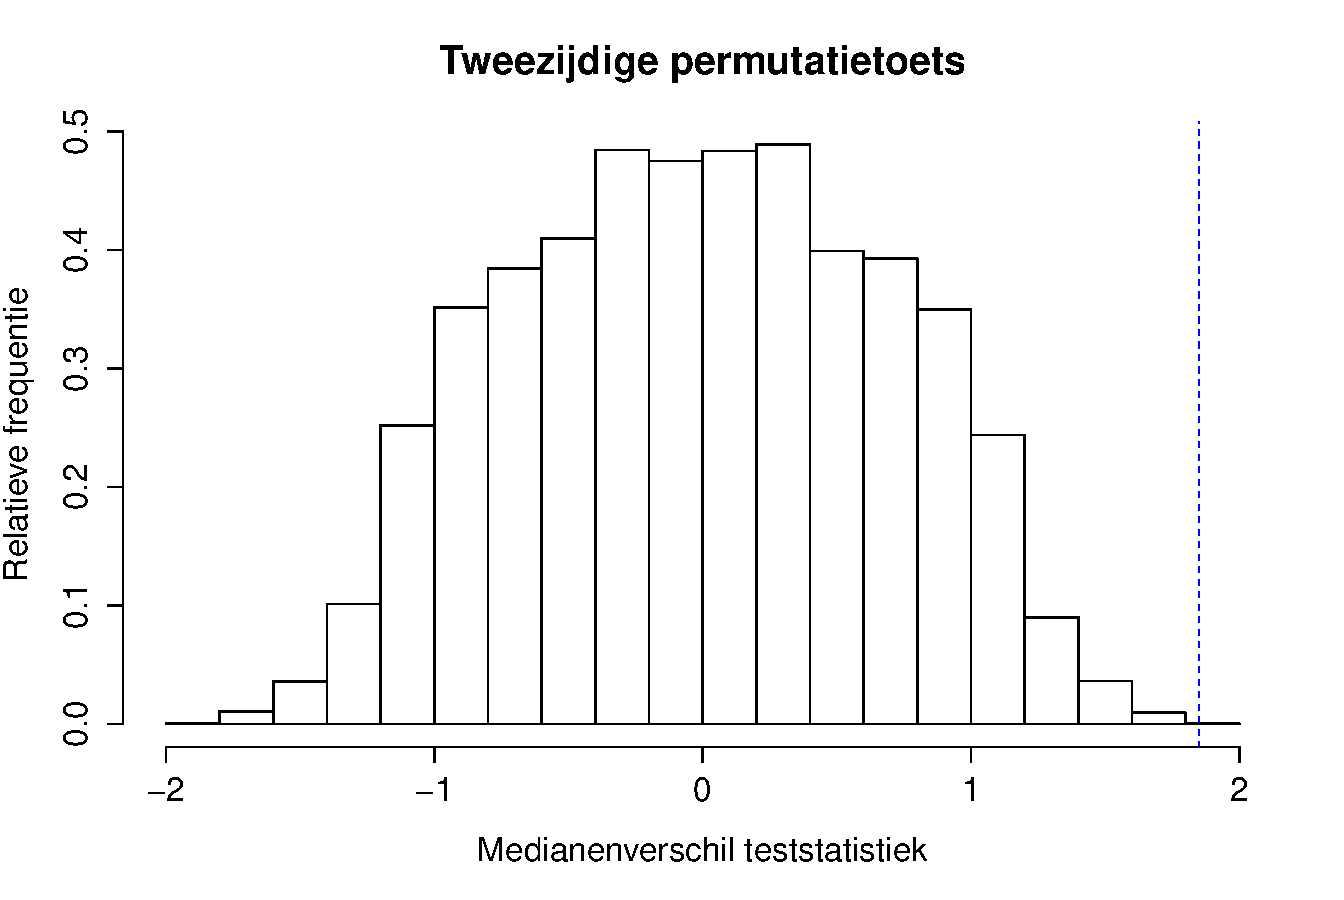
\includegraphics[scale=0.35]{perm_b.pdf}
			\caption{Permutatieverdeling voor de diameter groei bij bomen met en zonder competitie}
			\label{permb}
		\end{subfigure}
	\end{center}
	\caption{Barplot en permutatieverdeling van vraag 1b}
\end{figure}
\begin{wrapfigure}{R}{0.5\textwidth}
	\begin{center}		
		\vspace{-0.5cm}
		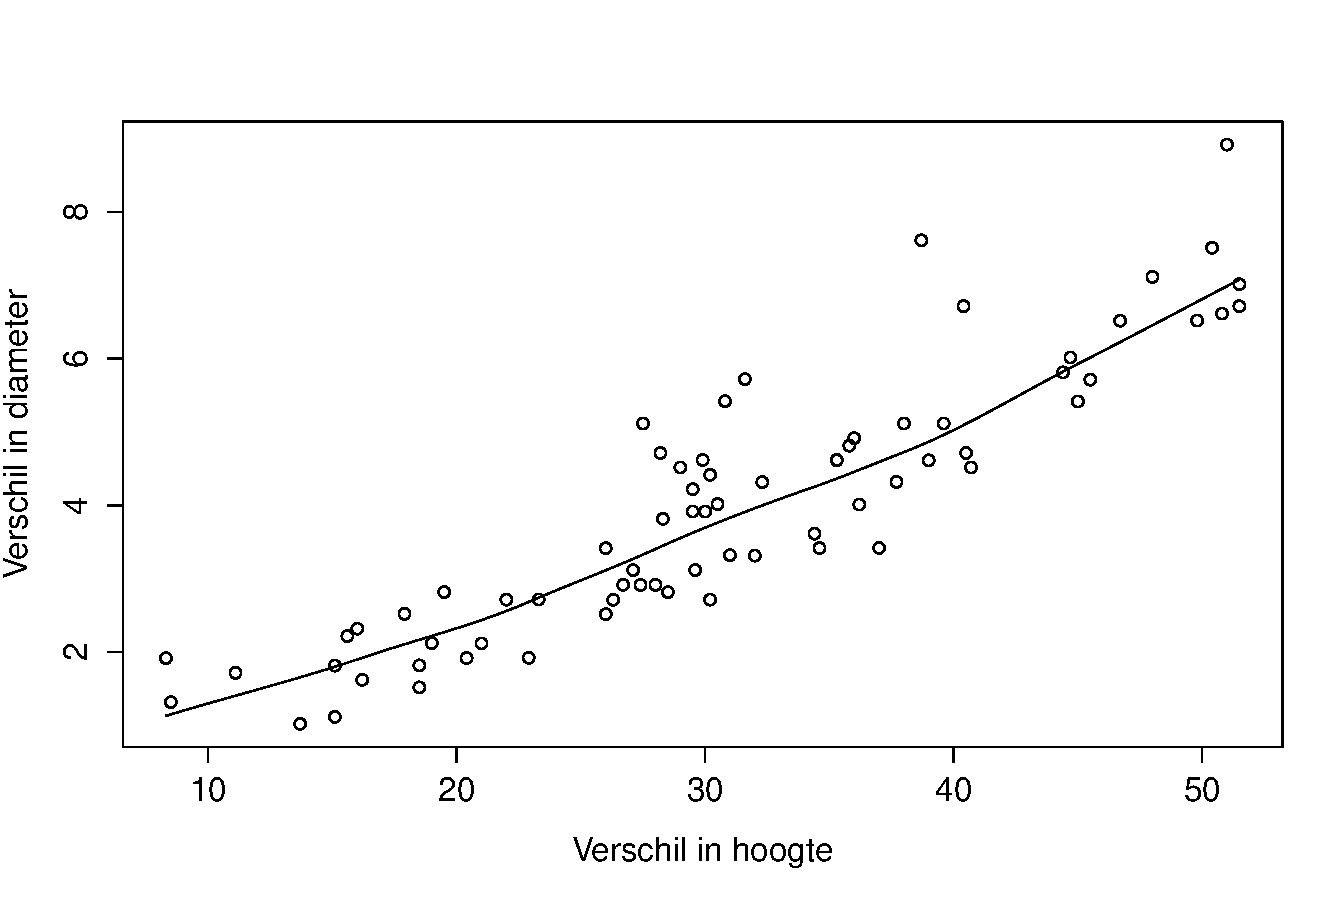
\includegraphics[scale=0.45]{scatter_c.pdf}
		\caption{Lineair verband tussen toename in diameter en toename in hoogte}
		\label{scatc}
		\vspace{-0.5cm}
		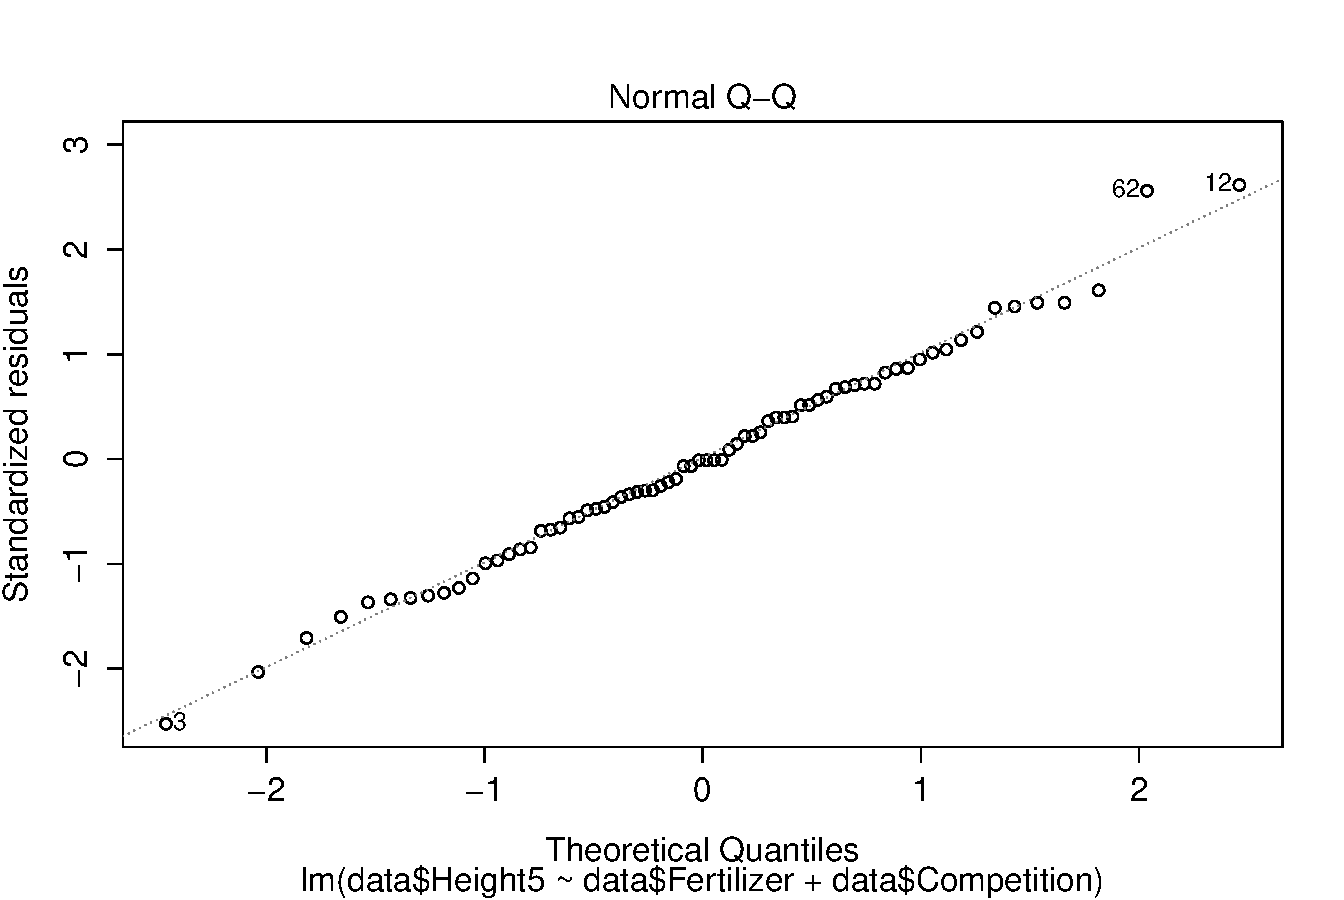
\includegraphics[scale=0.4]{qqplot_d.pdf}
		\caption{Symmetrische verdeling van het model}
		\label{qqplotd}
		\vspace{-0.5cm}
	\end{center}
\end{wrapfigure}
\subsection*{c}
Hier gaan we de associatie tussen de verschillen uit opgaves \textbf{a} en \textbf{b} bekijken. Aangezien deze beide continue variabelen zijn drukken we de associatie uit aan de hand van de covariantie, deze is $17.82$. We kunnen ook gemakkelijk de correlatie berekenen, deze is $0.90$. Aan de hand van deze twee waarden kunnen we beslissen dat de associatie groot is. Aangezien we echter niet weten hoe representatief onze steekproef is kunnen we de associatie niet precies bepalen. We kunnen dit ook visualiseren in een scatterplot met een smoother curve, deze is te zien in figuur \ref{scatc}. Deze curve lijkt op een rechte, wat wil zeggen dat er een lineair verband is tussen de toename van de lengte en deze van de diameter. In combinatie met de hoge waarde voor de correlatie kunnen we zeggen dat er een sterk linear verband is tussen de twee variabelen. Dit is echter data voor onze steekproef en niet voor de populatie.

\subsection*{d}
We stellen hiervoor een lineair regressie model op. Uit de summary van het model zien we dat het niet bemesten een negatieve invloed (schatting van $-14.772$) heeft op de groei en dat het afwezig zijn van competitie een positieve invloed (schatting van $10.917$) heeft. 

% Dirty hack to fix layout after using wrapfigures
\begin{wrapfigure}{R}{0pt}
\end{wrapfigure}
We zien op de Q-Q plot (figuur \ref{qqplotd}) dat er bijna geen afwijking van normaliteit is. In combinatie met de determinatie co\"effici\"ent, die $0.66$ is, kunnen we zeggen dat het model dus redelijk kwaliteitsvol is. De p-waarde is extreem laag, waardoor we kunnen beslissen dat de schattingen zeker goed zijn. % TODO: QQplot uitleggen

\subsection*{e}
Hierbij trekken we gewoon \textbf{Height0} van \textbf{Height5} af. We bekomen terug dat niet bemesten negatief is en dat de afwezigheid van competitie positief is voor de groei van de bomen. De determinatie co\"effici\"ent is $0.67$, net iets hoger dus het model is net iets beter.
\subsection*{f}
We zien een schatting voor de gemiddelde hoogtes voor de vier variabelen in de tabel hieronder.\\ \\
\begin{tabular}{r|c|c}
&Bemest&Onbemest\\
\hline
Competitie&$33.06$&$18.35$\\
\hline
Geen competitie&$43.52$&$28.81$\\
\end{tabular}
\section*{Opgave 2}
\subsection*{a}
Bij deze opgave is het belangrijk op te merken dat er gevraagd wordt naar een percentage binnen de populatie, het is dus niet voldoende het percentage uit te rekenen voor de steekproef. Om dit percentage te berekenen maken we gebruik van een $95\%$betrouwbaarheidsinterval, we doen dit aan de hand van de formule in de cursus. We bekomen dat dit interval $[0.5676, 0.7092]$ is. We kunnen dus met $95\%$ zekerheid stellen dat $56.76\%$ tot $70.92\%$ van de vrouwelijke degenkrabben in de de populatie over minstens \'e\'en satelliet beschikt tijdens de paringsperiode. Aangezien het percentage aan vrouwelijke krabben met een satelliet in onze steekproef $64.16\%$ is, is dit een representatieve steekproef.

\begin{wrapfigure}{r}{0.5\textwidth}
	\begin{center}		
		\vspace{-1cm}
		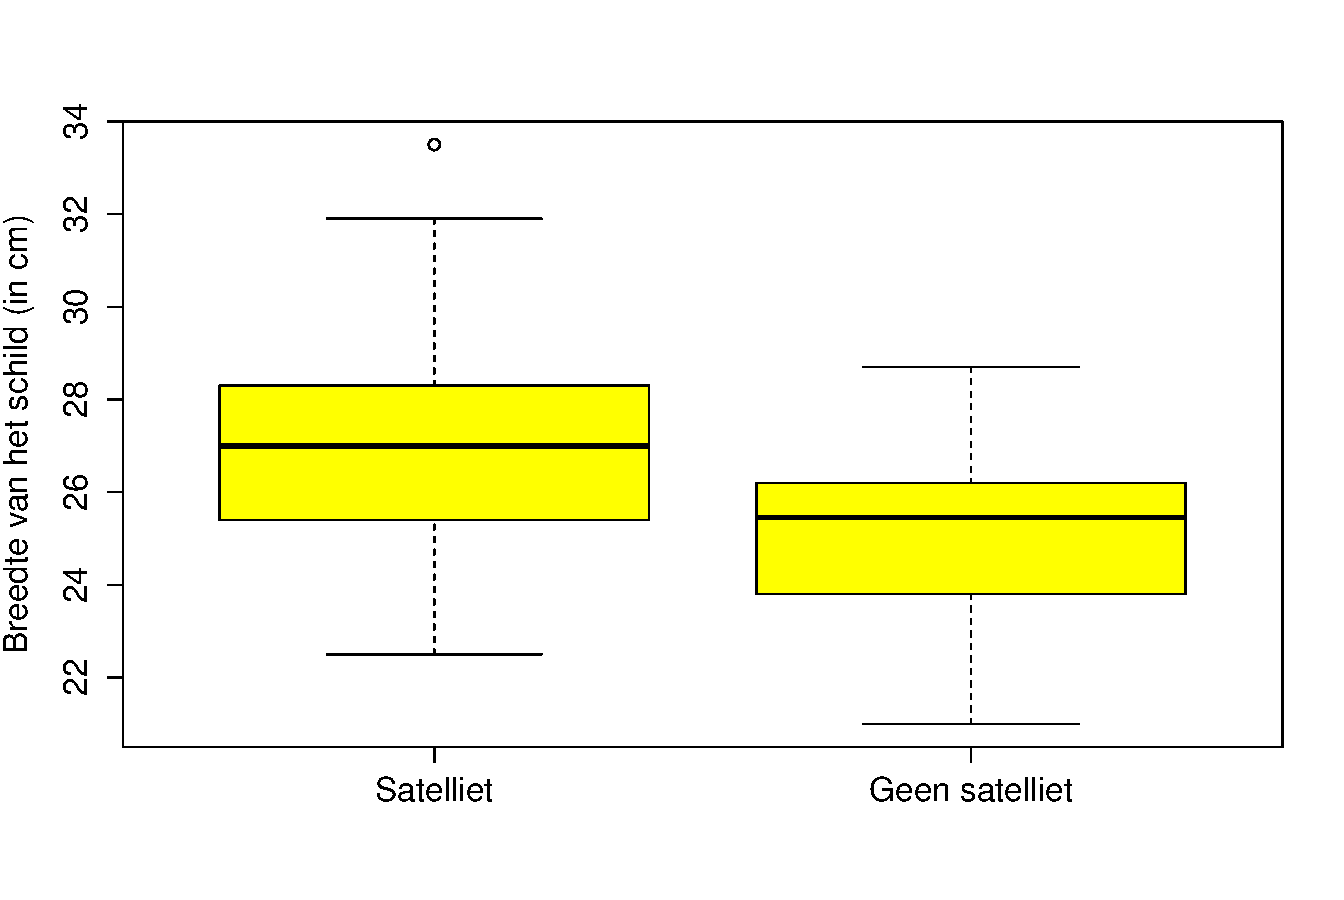
\includegraphics[scale=0.45]{box_b.pdf}
		\caption{Verschil in grootte van het schild bij vrouwtjes met en zonder satelliet}
		\label{boxb}
	\end{center}
\end{wrapfigure}
\subsection*{b}
De aanwezigheid van satellieten hangt inderdaad af van de grootte van het schild. Dit is duidelijk te zien in de boxplot op figuur \ref{boxb}. Om te weten in hoeverre deze verschilt doen we de t-test van Welch. Deze heeft als $H_0$ dat beide gemiddeldes (de gemiddelde van de schildgrootte van vrouwtjes met en zonder satellieten) gelijk zijn. $H_A$ stelt dan dat de gemiddeldes niet gelijk zijn. De p-waarde is $9.495 * 10^{-9}$, dit levert een overtuigend bewijs tegen de nulhypothese. 
% Dirty hack to fix layout after using wrapfigures
\begin{wrapfigure}{R}{0pt}
\end{wrapfigure}

Hierdoor kunnen we de nulhypothese verwerpen ten voordele van de alternatieve hypothese. Het betrouwbaarheidsinterval dat we bekomen met de t-test is $[1.19, 2.33]$. Vrouwtjes met satellieten hebben dus een schild dat $1.19$ tot $2.33$ cm groter is dan vrouwtjes zonder satellieten.
\subsection*{c}
Voor dit model op te stellen gebruiken we een lineaire en een kwadratische discriminant analyse. We vergelijken dan welke de beste is. We gebruiken ook leave-one-out cross-validation. Aan de hand van de tabellen kunnen we zien dat er bij de lineaire analyse met cross-validation een predictiefout is van $29.48\%$ en bij de kwadratische met cross-validation een van $31.79\%$. Voor de lineaire zonder cross-validation vinden we een schijnbare predictiefout van $28.90\%$ en voor de kwadratische zonder cross-validation $29.48\%$. De predictiefouten bij de schattingen met cross-validation liggen hoger dan die zonder, ze overfitten dus de training dataset wat leidt tot een instabielere classificatieregel die minder betrouwbare predicties oplevert. Op basis van de leave-one-out cross-validation schattingen van de predictiefout kunnen we besluiten dat de lineaire discriminant analyse stabielere resultaten oplevert dan de kwadratische.
\\\\
\begin{center}
\begin{tabular}{r|c|c}
&FALSE&TRUE\\
\hline
FALSE&$27$&$15$\\
\hline
TRUE&$35$&$96$\\
\end{tabular}
\captionof{table}{Misclassificatietabel voor lineaire discriminant analyse}

\begin{tabular}{r|c|c}
&FALSE&TRUE\\
\hline
FALSE&$30$&$19$\\
\hline
TRUE&$32$&$92$\\
\end{tabular}
\captionof{table}{Misclassificatietabel voor lineaire discriminant analyse}

\begin{tabular}{r|c|c}
&FALSE&TRUE\\
\hline
FALSE&$26$&$15$\\
\hline
TRUE&$36$&$96$\\
\end{tabular}
\captionof{table}{Leave-one-out cross-validation misclassificatietabel voor lineaire discriminant analyse}

\begin{tabular}{r|c|c}
&FALSE&TRUE\\
\hline
FALSE&$28$&$21$\\
\hline
TRUE&$34$&$90$\\
\end{tabular}
\captionof{table}{Leave-one-out cross-validation misclassificatietabel voor kwadratische discriminant analyse}
\end{center}
\newpage
\section*{Appendix}
Hieronder vindt u de gebruikte R code met extra informatie in commentaar. 
\begin{framed}
\lstinputlisting[language=R]{Oplossingen.R}
\end{framed}
\end{document}